
\PassOptionsToPackage{unicode}{hyperref}
\PassOptionsToPackage{naturalnames}{hyperref}
\documentclass{beamer} 
%\usepackage{babel}
%\usepackage[utf8]{inputenc}


%%% FONT SELECTION %%%%%%%%%%%%%%%%%
%%% we choose a sans font %%%%%%%%%%
\usepackage{kmath,kerkis} 
%\usepackage[default]{gfsneohellenic} 
%%%%%%%%%%%%%%%%%%%%%%%%%%%%%%%%%%%%

\usepackage{color}
\usepackage{amsmath}
\usepackage{amssymb}

\usepackage{epstopdf}
\usepackage{graphicx}
\graphicspath{{./images/presentation}}

%%
% load TEI-Pel - specific layout
\usepackage{TeiPel_En_Beamer_Layout}
\setTeipelLayout{draft,newlogo}% options: "draft", "newlogo"



% Thesis Info - first page 
	% title
		\title[Gravimetric Sensing Aided by Radiation Cooling]{Gravimetric Sensing Aided by Radiation Cooling}		
    %\author
		\author[Yishai Arieli]{Yishai Arieli}
	% supervisor	
		\supervisor{Supervisor}{Professor Howell}
	% date
		\presentationDate{October 22, 2021}


\begin{document}

% typeset front slides
	\typesetFrontSlides

% Your Slides Start here:
\section{Theoretical background}
\subsection{Torsional pendulum}
% frame 1
\begin{frame}{Harmonic oscillator}
	\begin{center}		
		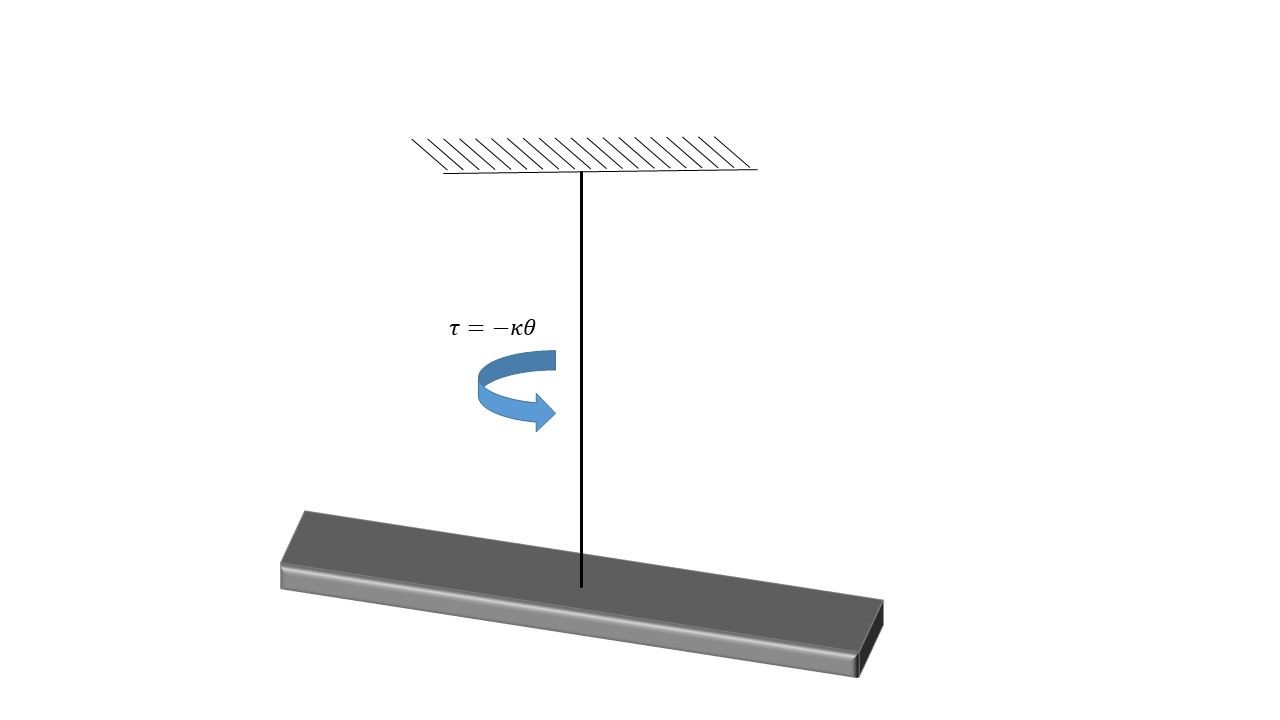
\includegraphics[width=0.4\textwidth,keepaspectratio]{torsion_pendulum_powerpoint.jpg}
    \end{center}
	\begin{itemize}

		\item Torsional pendulum is an angular harmonic oscillator with a restoring torque, made of a mass hung by a string. 
		\pause
		\item Undamped oscillator; harmonic oscillations without decay.
		\item Damped oscillator; there is also a damping torque $\tau = -b\dot{\theta}$.
		
	\end{itemize}
\end{frame}
% frame 2
\begin{frame}{Damped oscillator}
	\begin{center}		
		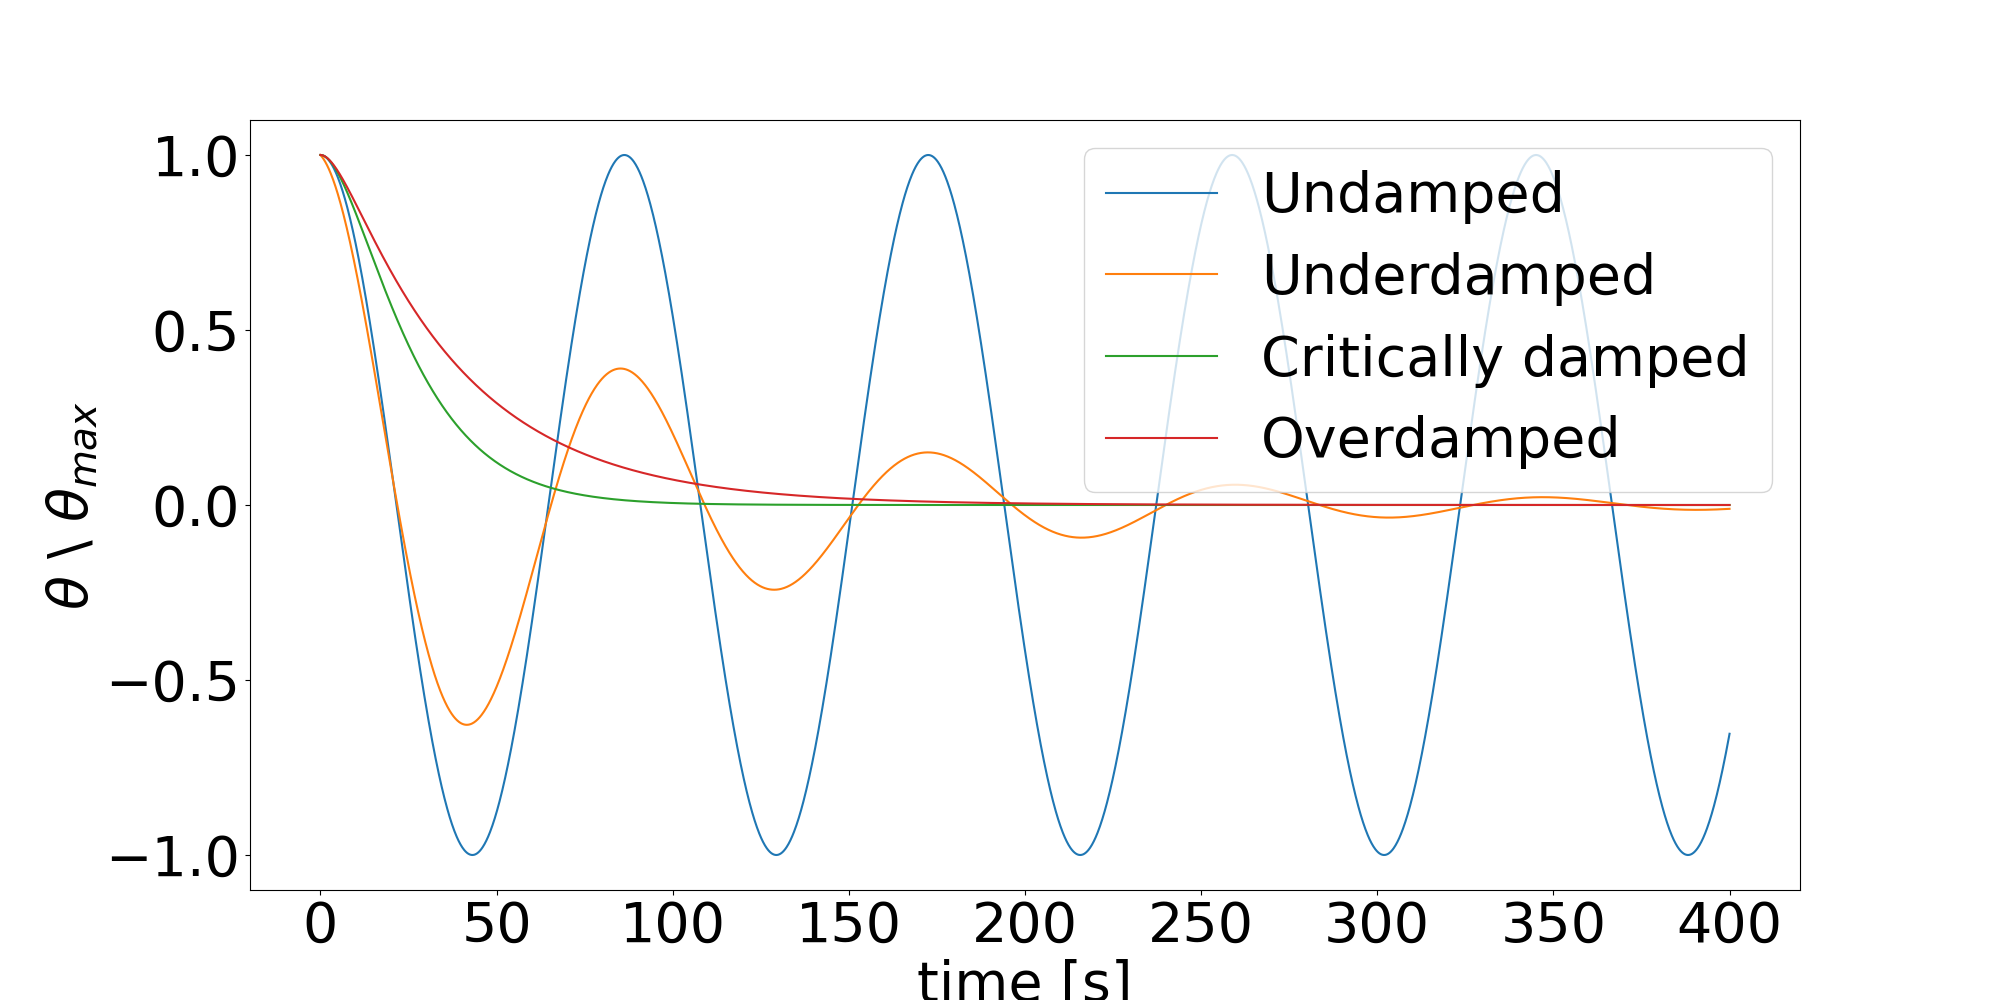
\includegraphics[width=0.55\textwidth,keepaspectratio]{damp.png}
    \end{center}
	\begin{itemize}
		
		\item Underdamped; oscillations amplitude decreases in time while oscillating with a lower frequency.
		\item Critically damped; exponential decay to equilibrium.
		\item Overdamped; exponential decay with longer damping time. 
		\pause
		\item Driven oscillator; there is also a time-dependent torque $\tau(t)$.
	\end{itemize}
	\hyperlink{frame:Gravitational field}{>>} 
\end{frame}

% frame 3 - skip
\begin{frame}{Damped oscillator}
	\framesubtitle{Damped equation}
	\begin{center}		
		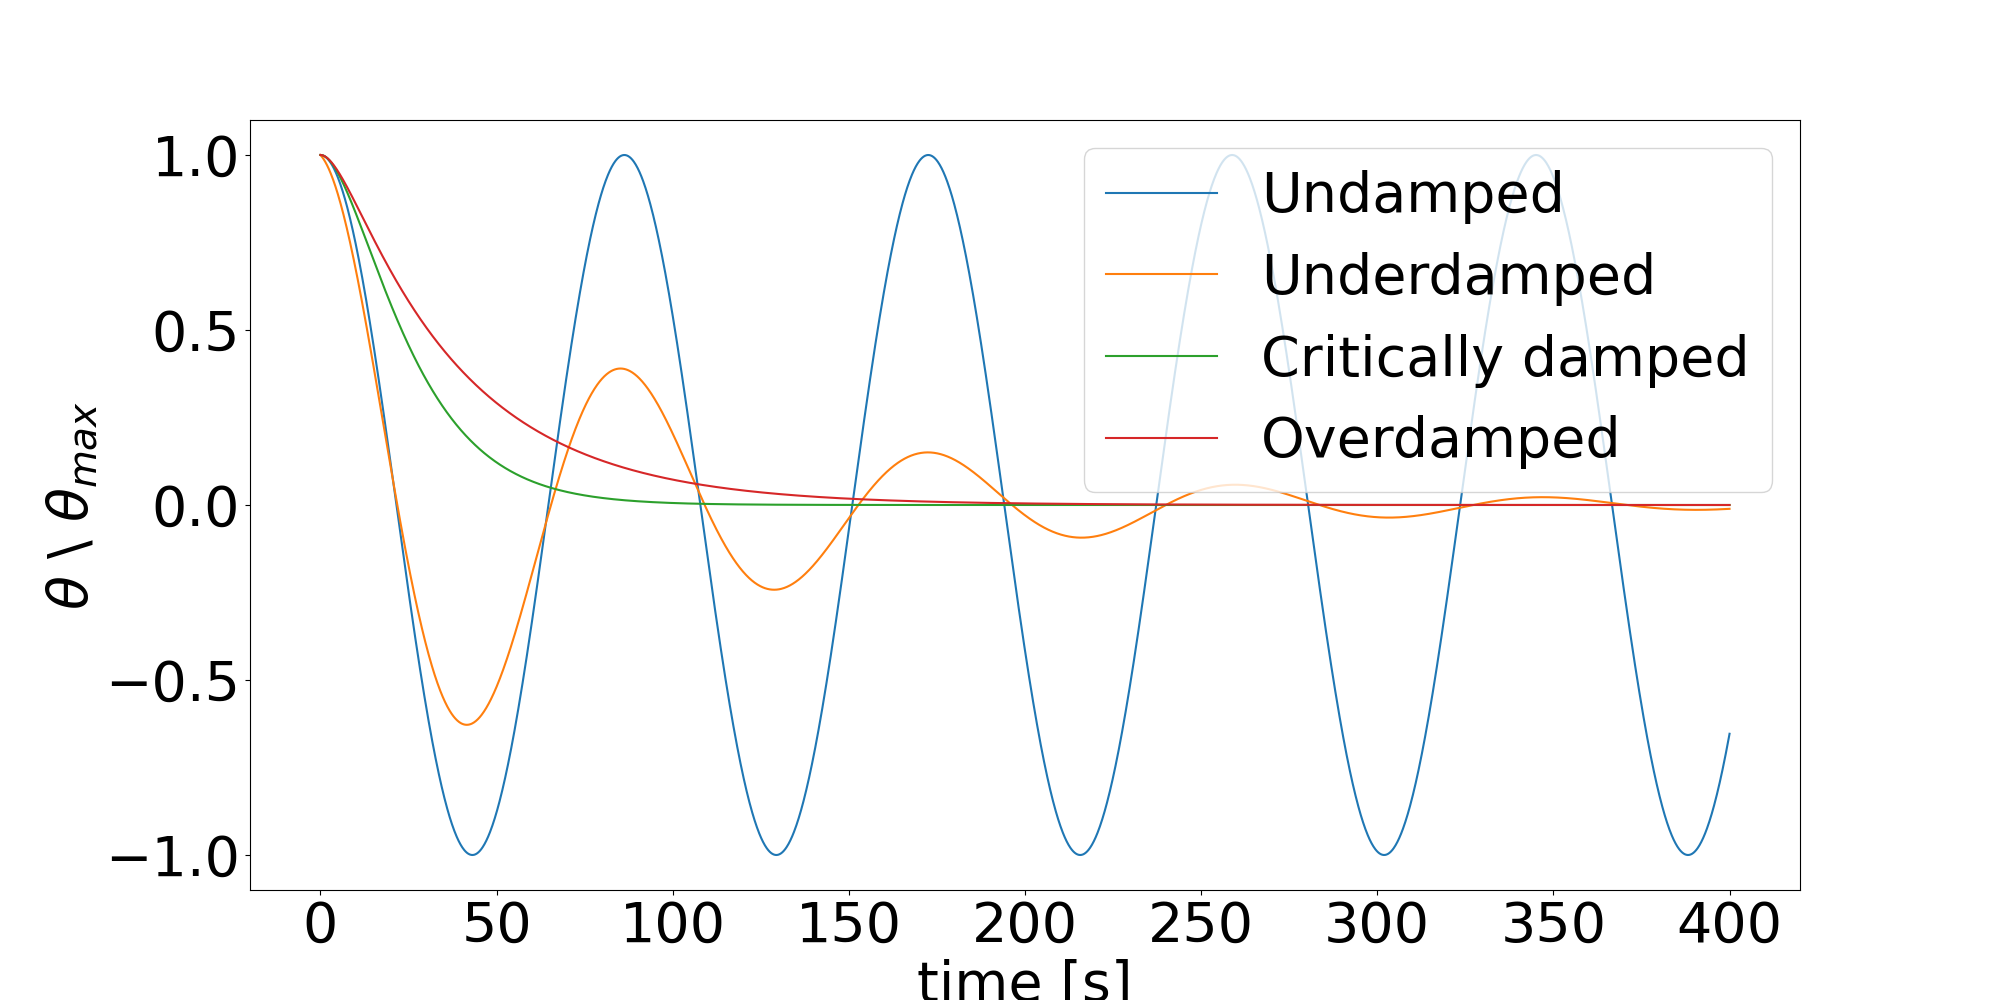
\includegraphics[width=0.5\textwidth,keepaspectratio]{damp.png}
    \end{center}
	\begin{itemize}	
		\item The pendulum is a damped oscillator if there is a damping torque opposite to the angular velocity $\tau = -b\dot{\theta}$.
		\item The damped motion is given by $\ddot{\theta} + 2\xi\omega_0\dot{\theta} + \omega_0^2\theta = 0$.
		\item The damping ratio, $\xi$, determines the oscillator's motion: underdamped, critically damped or overdamped.
	\end{itemize}
	
	
\end{frame}


\subsection{Gravity measurement}
% frame 1
\begin{frame}{\hypertarget{frame:Gravitational field}{Gravitational field}}
	\begin{center}		
		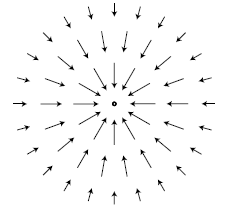
\includegraphics[width=0.3\textwidth,keepaspectratio]{gravity.png}
    \end{center}
	\begin{itemize}
		\item Newton's law of universal gravitation: $\overrightarrow{F} = \frac{GMm}{r^2}\hat{r}$
		\item The field vectors point towards the mass: $\overrightarrow{g}(M) = \frac{GM}{r^2}\hat{r}$ 
		\item Since the gravitational constant is small, the force is weak.
		\end{itemize}
\end{frame}
% frame 2
\begin{frame}{Cavendish apparatus}
	\begin{center}		
		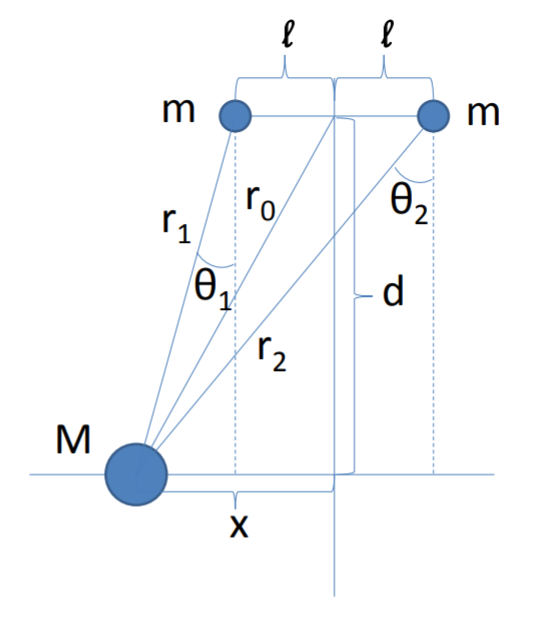
\includegraphics[width=0.25\textwidth,keepaspectratio]{Cavendish apparatus.PNG}
    \end{center}
	\begin{itemize}
		\item Cavendish apparatus measures the test mass $M$ gravitational torque using a torsional pendulum.
		\pause
		\item Mass $M$ attracts both masses $m$; creating a net gravitational torque.
		\item There are both gravitational torque and a restoring torque.
		\pause
		\item The average equilibrium angle: $\overline{\theta} = \frac{\tau_g}{\kappa} \approx \frac{3GT^2cos\theta sin\theta}{4\pi^2 } \cdot \frac{M}{r_0^3}$.

	\end{itemize}
	\hyperlink{frame:Gravimetric sensing}{>>} 
\end{frame}
% frame 3 - skip
\begin{frame}{Cavendish apparatus}
	\framesubtitle{Net torque}
	\begin{center}		
		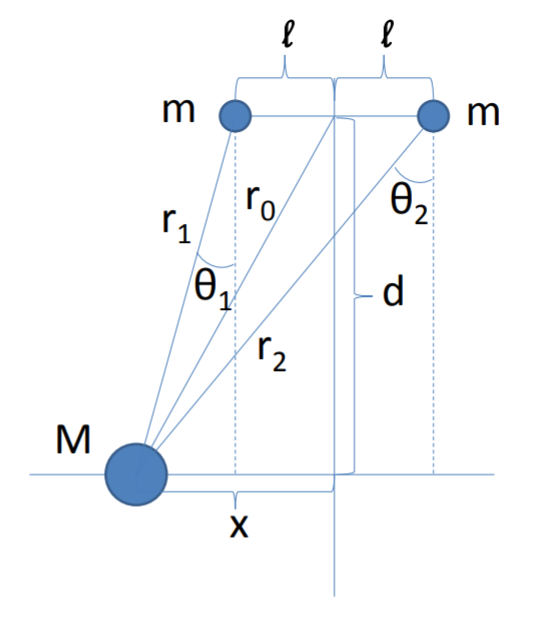
\includegraphics[width=0.25\textwidth,keepaspectratio]{Cavendish apparatus.PNG}
    \end{center}
	\begin{itemize}
		\item The net gravitational torque is the sum inverse torques, one from each mass: $\tau_g = l \cdot F(r_1) \cdot cos\theta_1 - l \cdot F(r_2) \cdot cos\theta_2$
		\item If $l<<d,x,r_0$ the net torque can be approximated to: $\tau_g =  \frac{6l^2GmMxd} {r_0^5} = \frac{6l^2GmM sin\theta cos\theta}{r_0^3}$
		\item Where the tilt angle is $\theta_1 \approx \theta_2 \approx \theta$.
	\end{itemize}
	\hyperlink{frame:Gravimetric sensing}{>>} 
\end{frame}
% frame 4 - skip
\begin{frame}{Cavendish apparatus}
	\framesubtitle{Approximation}
	\begin{center}		
		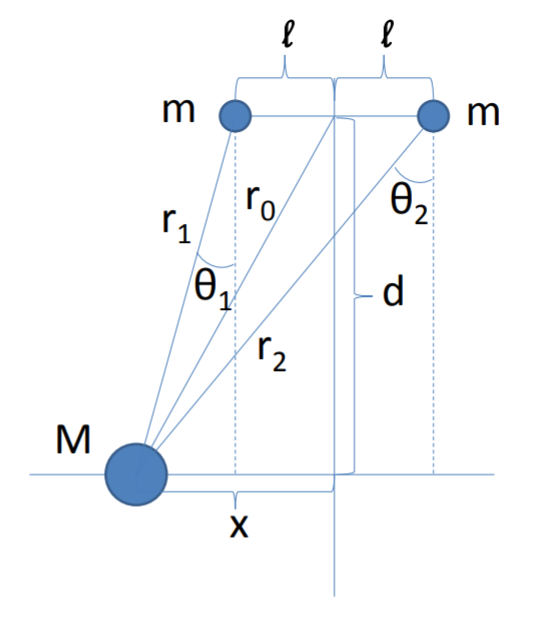
\includegraphics[width=0.2\textwidth,keepaspectratio]{Cavendish apparatus.PNG}
    \end{center}
	\begin{itemize}
		\item The net gravitational torque: $\tau_g =  l d GmM(\frac{1}{r_1^3} - \frac{1}{r_2^3})$.
		\item Defining the function: $h(l) = \frac{1}{(d^2 +(x-l)^2)^{3/2}}$.
		\item If $l<<d,x,r_0$ approximation: $h(l)-h(-l)\approx h'(0)\cdot 2l = \frac{6lx}{r_0^5}$.
		\item the net torque is proportional to the difference: $\tau_g = l d GmM[h(l)-h(-l)]\approx \frac{6l^2GmMxd} {r_0^5}$.
	\end{itemize}
	\hyperlink{frame:Gravimetric sensing}{>>} 
\end{frame}
% frame 5 - skip
\begin{frame}{Cavendish apparatus}
	\framesubtitle{Simple harmonic oscillator}
	\begin{center}		
		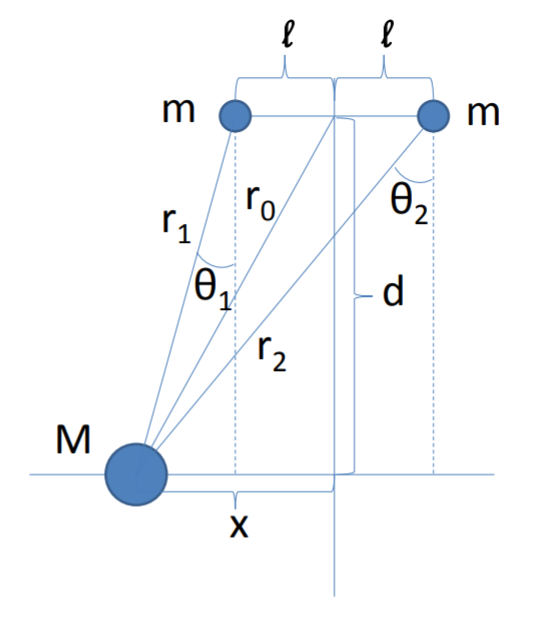
\includegraphics[width=0.25\textwidth,keepaspectratio]{Cavendish apparatus.PNG}
    \end{center}
	\begin{itemize}
		\item Assuming no damping force (simple harmonic motion).
		\item At equilibrium, the torques cancel each other out $\tau_g =  \kappa\theta$.
		\item The average equilibrium angle: $\overline{\theta} = \frac{\tau_g}{\kappa} \approx \frac{3GT^2cos\theta sin\theta}{4\pi^2 } \cdot \frac{M}{r_0^3}$.
		
	\end{itemize}
	\hyperlink{frame:Gravimetric sensing}{>>} 

\end{frame}
% frame 6
\begin{frame}{\hypertarget{frame:Gravimetric sensing}{Gravimetric sensing}}
	
	\begin{itemize}
		\item Time integration reduces measurement noises. 
		\item SNR is the limiting factor for the measurement sensitivity.		
		\pause
		\item Integration at high frequencies is faster with better SNR.
		\item SNR frequency dependency is a significant challenge with low frequency gravimetric sensing.

	\end{itemize}
\end{frame}


\subsection{Noises and damping}
% frame 1
\begin{frame}{Environmental noises}
	\begin{center}		
		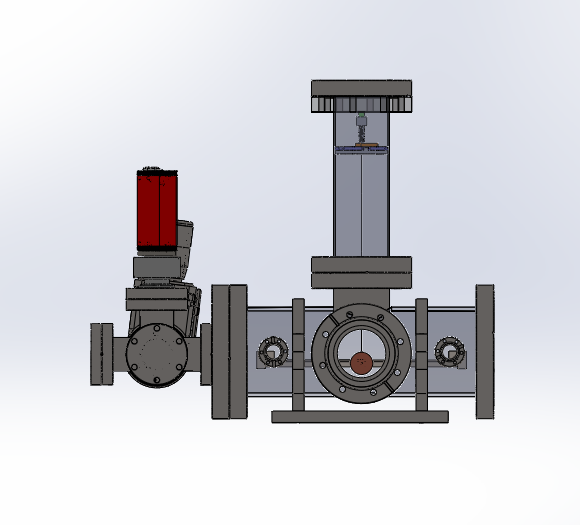
\includegraphics[width=0.4\textwidth,keepaspectratio]{total_chamber.png}
    \end{center}
	\begin{itemize}
		
		\item Environment cause pressure-dependent friction and noises (Brownian motion, acoustic waves, thermal flow).  
		\item Noise from environmental black body radiation.
		\item Unknown Magnetic noise from electronics.
		\pause
		\item System placed inside a vacuum chamber and acoustic box. 
			
	\end{itemize}
	\hyperlink{frame:Proportional–integral–derivative (PID) controller}{>>} 
\end{frame}
% frame 2 - skip
\begin{frame}{Environmental noises}
	\framesubtitle{Pressure and temperature dependent noises}
	\begin{itemize}
		\item An ideal gas has negligible inter-particle interactions.
		\item Brownian motion cause random collisions. 
		\item The kinetic energy of the gas particles: $ N<E_k> = \frac{3}{2} PV$.
		\item Acoustic waves are propagating with power of $10^{-22}AP^2$.
		\item Heat flow is the exchange of thermal energy between physical systems. The net power is: $p= A P c_v \Delta T \sqrt{\frac{M}{RT}} $.
		\item Net power from black body radiation is $p= A \sigma\epsilon[ T^4- T_0^4]$.
		
	\end{itemize}
	\hyperlink{frame:Proportional–integral–derivative (PID) controller}{>>} 
\end{frame}
% frame 3 - skip
\begin{frame}{Environmental noises}
	\framesubtitle{Friction}
	\begin{itemize}
		\item Friction, caused by drag force, decreases with pressure.		
		\item At higher pressures (turbulent flow); $F = -b(P)\cdot v^2 $.
		\item At lower pressures (gas with laminar flow), the drag force is given by Stokes' law: $F_{drag} =  -b(P)\cdot v$.	
		
	\end{itemize}
	\hyperlink{frame:Proportional–integral–derivative (PID) controller}{>>} 
\end{frame}


% frame 4
\begin{frame}{\hypertarget{frame:Proportional–integral–derivative (PID) controller}{Proportional–integral–derivative (PID) controller}}
	\begin{center}		
		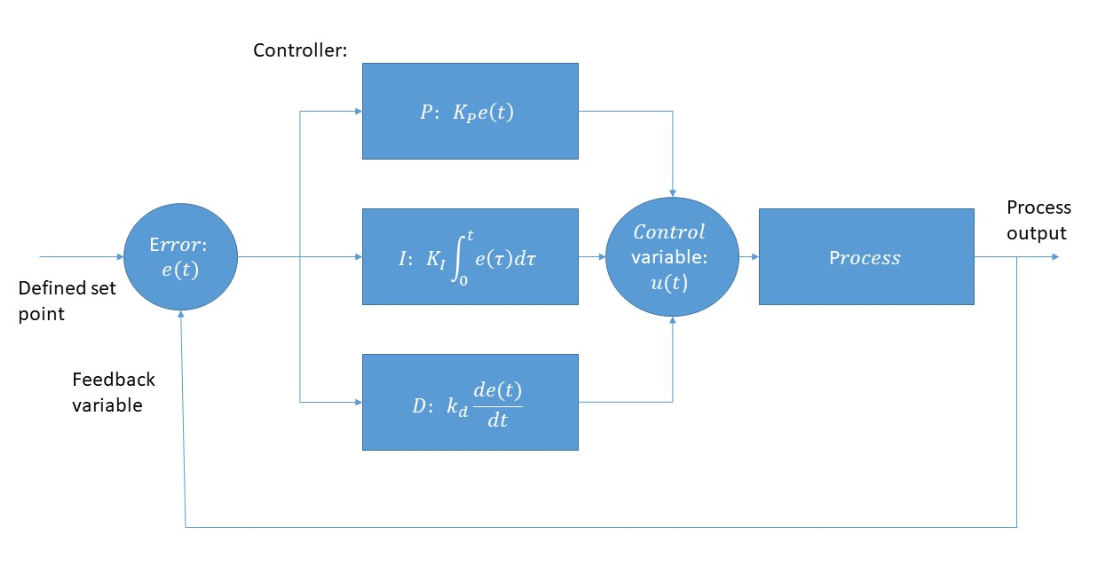
\includegraphics[width=0.6\textwidth,keepaspectratio]{pid_diagram_powerpoint.jpg}
    \end{center}
	\begin{itemize}	
		\item PID controller is a feedback based control system, for time continuous control of a process.
		\item The controller continuously calculates error from set point. 
		\pause
		\item The control is based on a proportional, integral and derivative response to the error (P-I-D).
	\end{itemize}
\end{frame}
% frame 5
\begin{frame}{PID response}
	\begin{center}		
		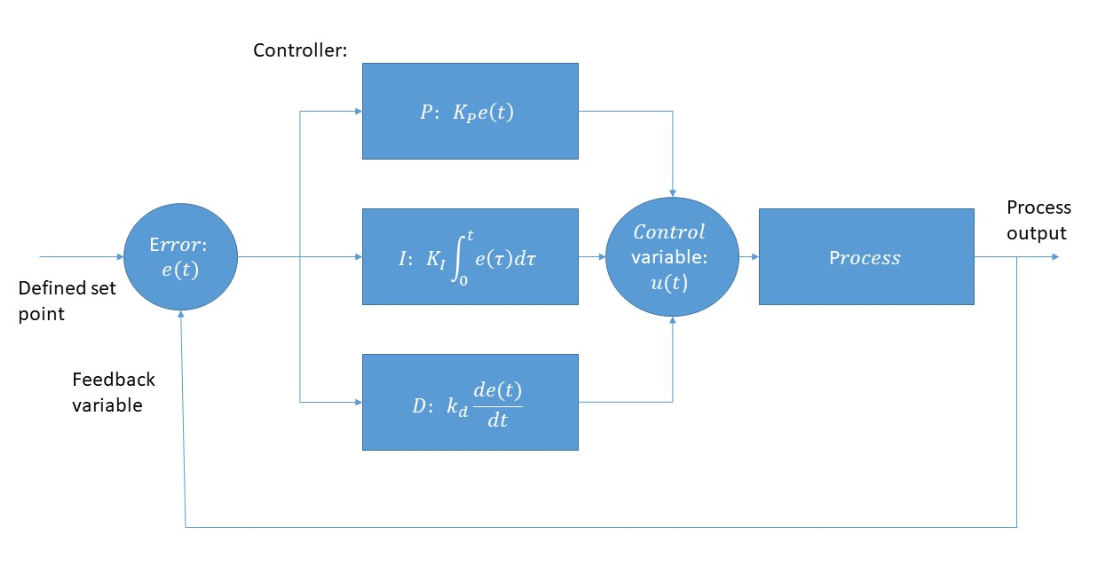
\includegraphics[width=0.6\textwidth,keepaspectratio]{pid_diagram_powerpoint.jpg}
    \end{center}
	\begin{itemize}
	
		\item Each response is modulated by a tunable gain. 
		\item The output is a weighted sum of the response terms.
		%\item $u(t) = K_P e(t)+K_I\int_{0}^{t}e(\tau)d\tau+K_D\frac{de(t)}{dt}$
		\pause
		\item The feedback applies an external correction to the process.	
		\item Over time error is minimized (damped motion).
	\end{itemize}
\end{frame}
% frame 6
\begin{frame}{\hypertarget{frame:Radiation tourqe}{Radiation tourqe}}
	
	\begin{itemize}		
		
		\item Incident light beam causes force on the surface, due to momentum exchange with the electromagnetic field.
		%\item The force depend on the relative angle, surface reflectance and absorbance and the incident light power.
		\pause
		\item With light perpendicular to a reflective surface $F  \approx\frac{2\eta\Theta}{{c}} $.
		\item Two light sources result with a modulated net tourqe.
		
	\end{itemize}
\end{frame}

\section{Thesis aims}
% frame 1
\begin{frame}{Experiment noises}
	\begin{center}		
		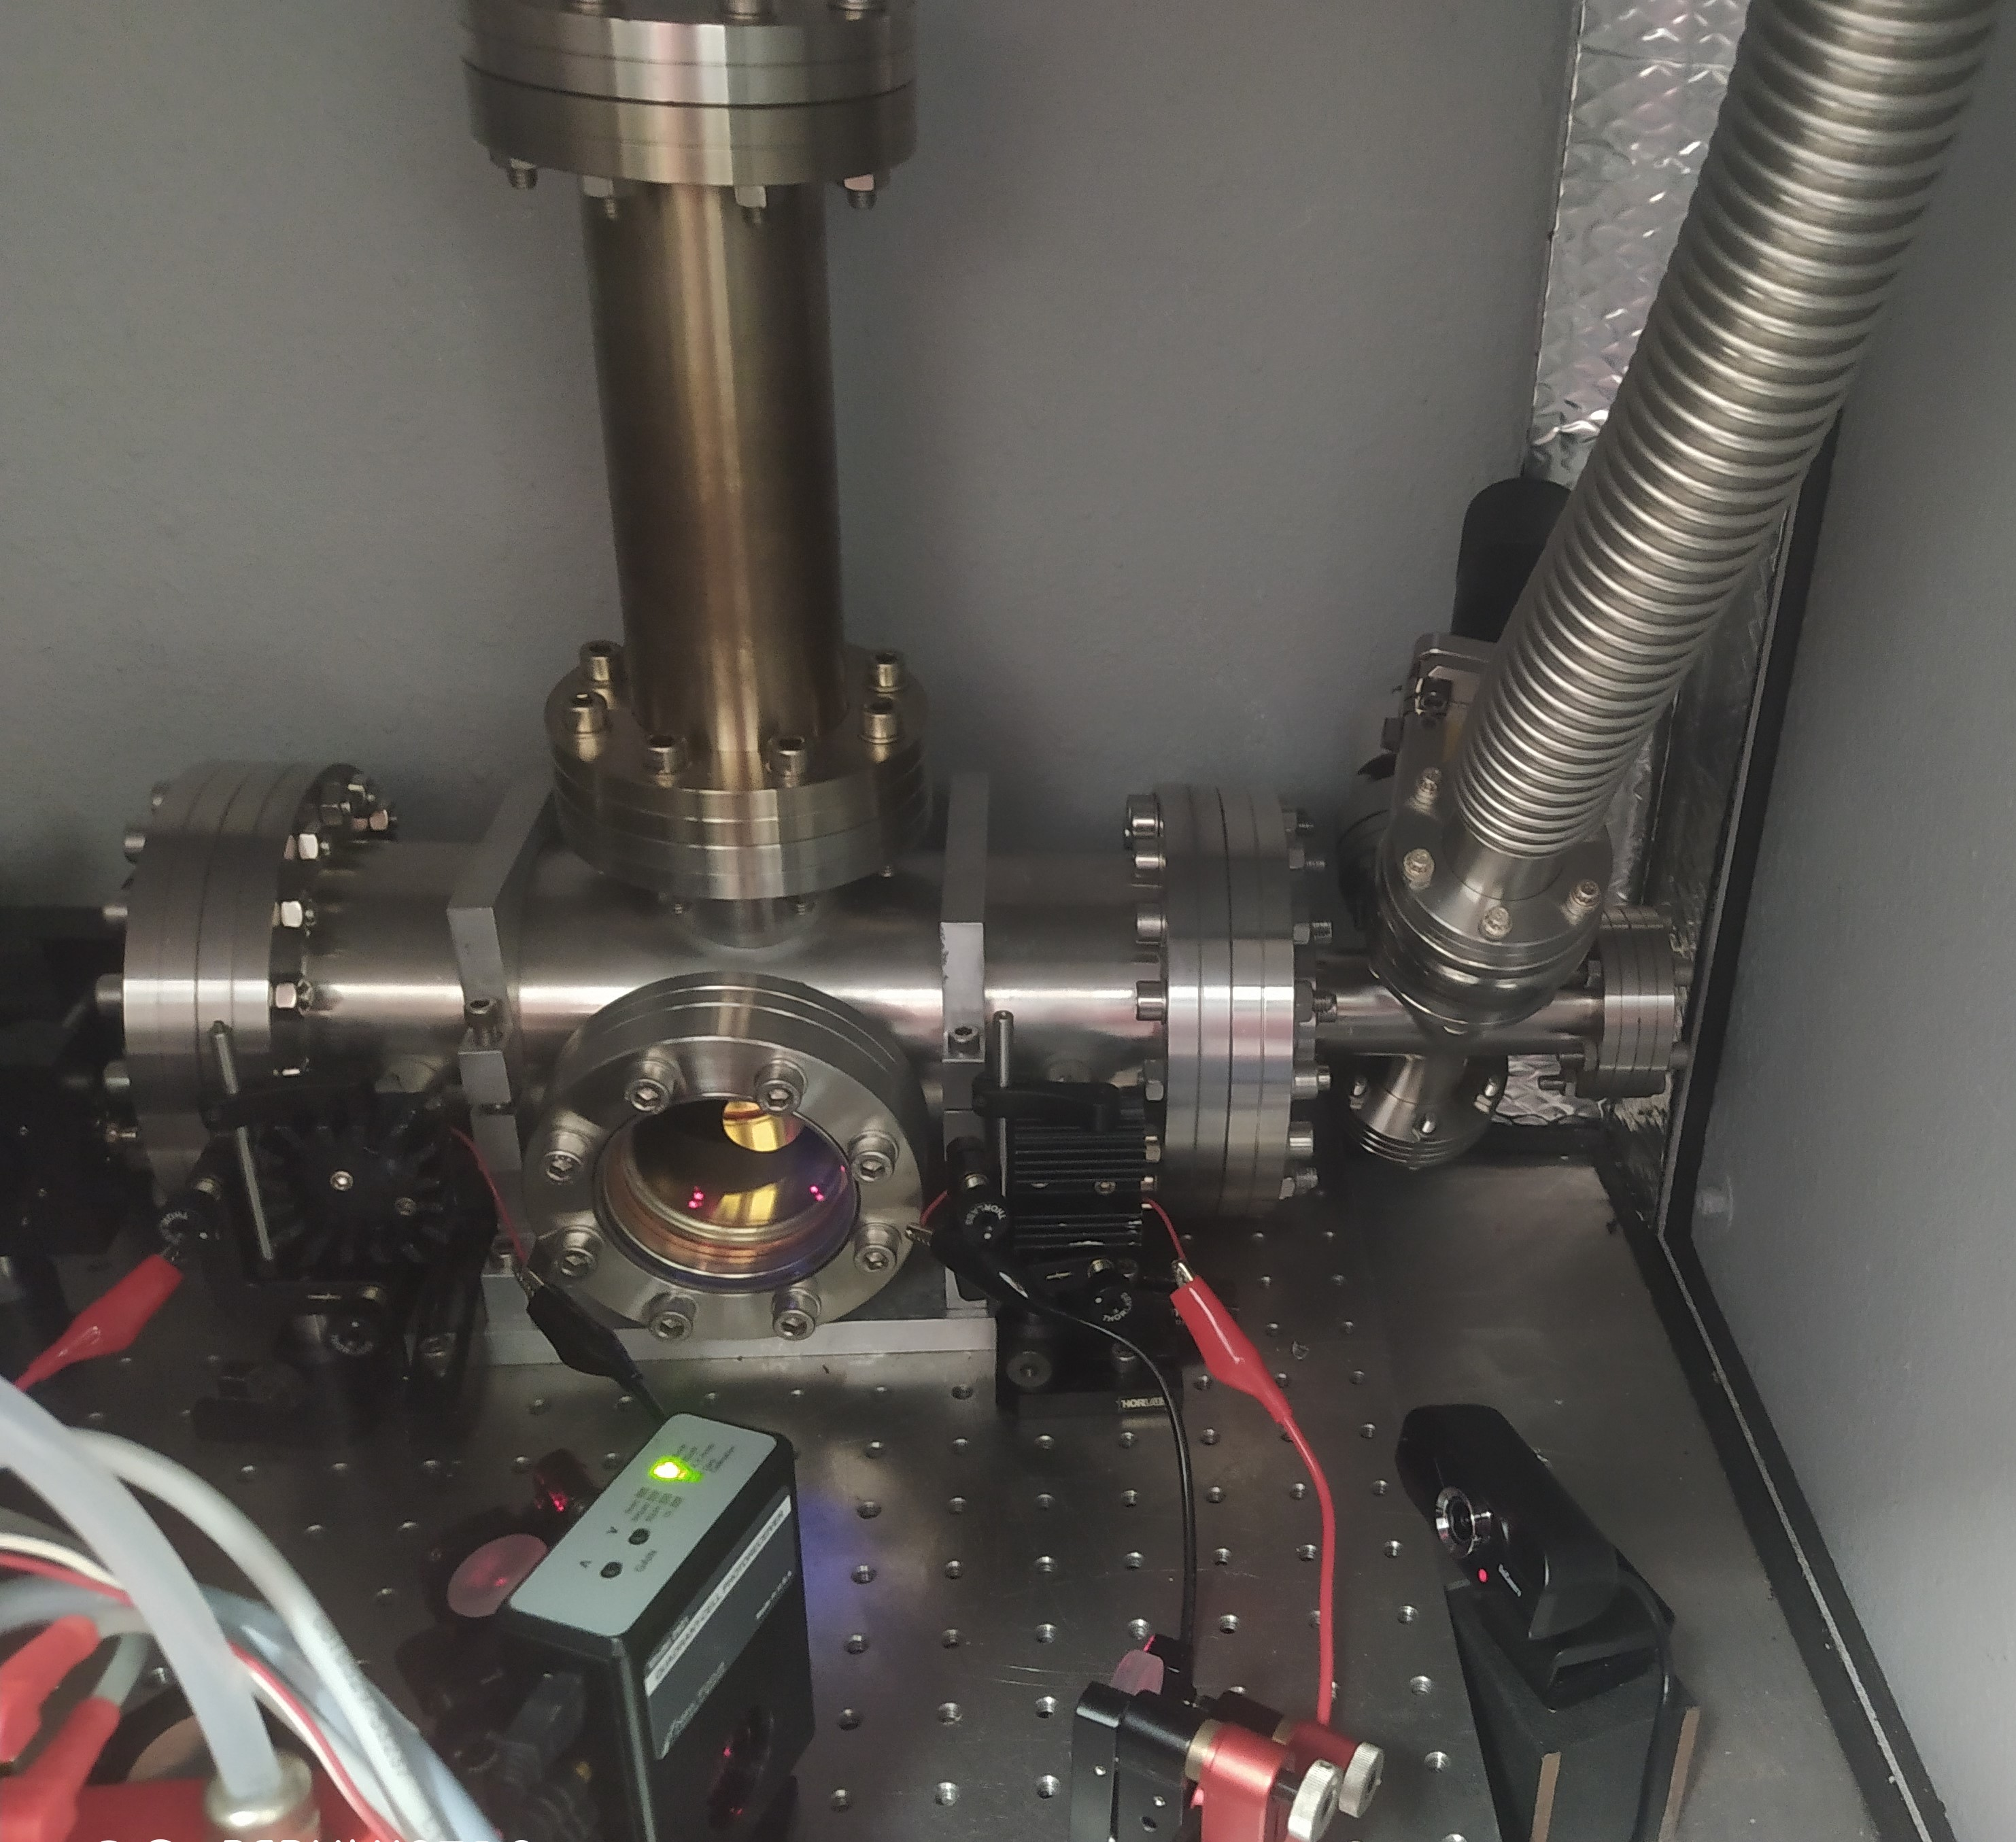
\includegraphics[width=0.3\textwidth,keepaspectratio]{actual system_crop.jpg}
    \end{center}
	\begin{itemize}
		
		\item Angle measurement is optical with a front mirror.
		\item Fundamental limits are: thermal uncertainty, shot noise. 
		\pause
		\item Reducing the uncertainty $\delta\theta$ enables higher sensitivity.
		\item When amplitude is damped under the thermal limit, PID is effectively lowering the temperature; $\delta\theta = \sqrt{\frac{k_B T}{\kappa}}$. 
		
		
	\end{itemize}
	\hyperlink{frame:Gravimetric measurement}{>>} 
\end{frame}
% frame 2 - skip
\begin{frame}{Experiment noises}
	\begin{itemize}
		\framesubtitle{Fundamental limits}
		\item Basic energy level quantum uncertainty: $delta\theta= \sqrt{\frac{\hslash\omega}{2\kappa}} \approx 10^{-16} [rad]$
		\item Quantum uncertainty due to thermal energy: $\delta\theta = \sqrt{\frac{k_B T}{\kappa}} \approx 4\cdot 10^{-8} [rad]$.
		\item Shot noise limit: $\delta\theta = \frac{1}{4\sqrt{2}\pi}\frac{\lambda}{L\sqrt{N}} \approx 10^{-14} [\frac{rad}{Hz}]$.
		
	\end{itemize}
\end{frame}

\begin{frame}{\hypertarget{frame:Gravimetric measurement}{Gravitational measurement}}
	\begin{itemize}
		
		
		\pause
		\item Introducing a new mass adds a constant new torque $\tau_g$. 
		\item The PID is compensating for the new error; response becomes mainly an inverse torque: $\tau_{PID}(t) \approx K_P\theta_g(t)$. 
		\item When integrating over short periods the gravitational angle is constant: $\overline{\theta}_g =  \frac{\int \tau_{PID}(t) dt}{ K_P \Delta t} $ allowing short integration time.
		
		
	\end{itemize}
\end{frame}

\section{Methods and results}
\subsection{System structure}
\begin{frame}{Experiment setup}
	\begin{center}		
			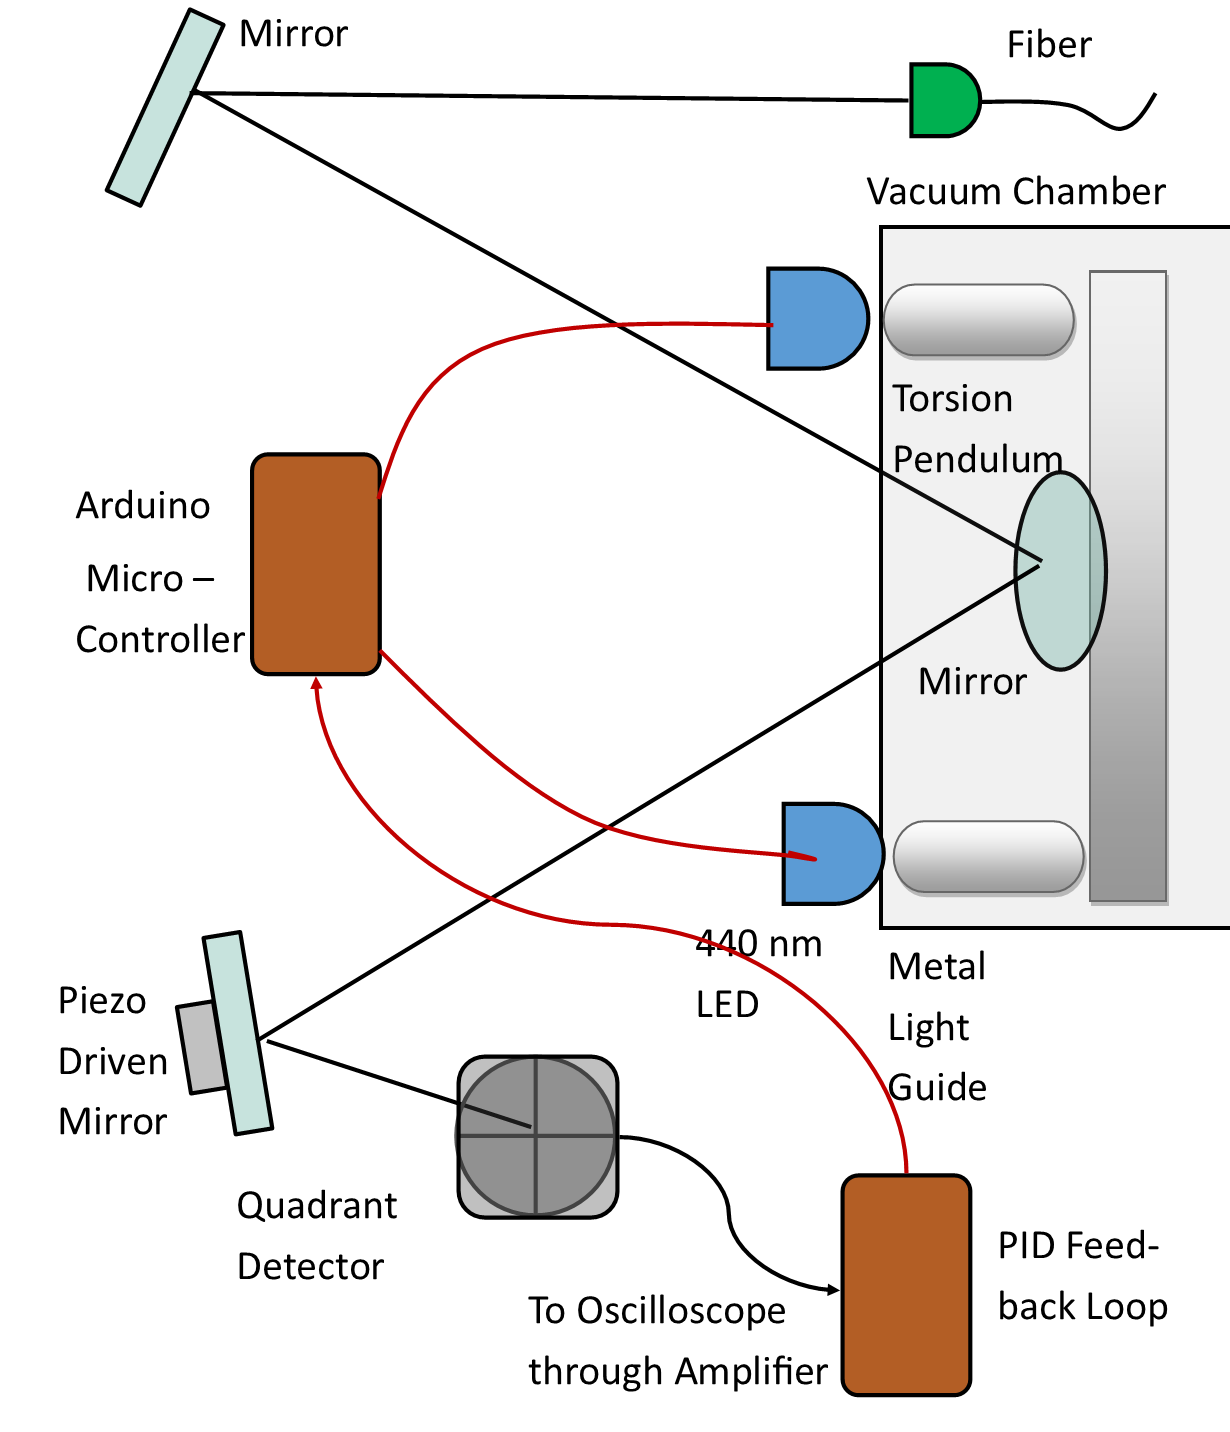
\includegraphics[width=0.3\textwidth,keepaspectratio]{setup cropped.png}
	\end{center}
	\begin{itemize}

		\item The torsional pendulum is placed inside a vacuum chamber, with angle measurement system and a feedback system. 
		\item Laser beam deflected by the pendulum's front mirror and detected by a quadrant detector.
		\pause
		\item Feedback of two LED light sources, modulated in real time by an Arduino controller; controlled by the PID loop.
		%\item The angle is read in real time by the PID algorithm; radiation torque is exerted by the LED's flux.
	
	\end{itemize}
	
\end{frame}

\begin{frame}{Experiment setup}
	\begin{center}		
		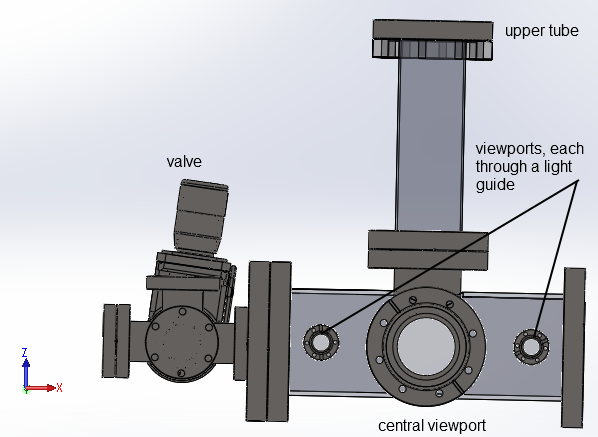
\includegraphics[width=0.4\textwidth,keepaspectratio]{chamber_front_names.PNG}
	\end{center}
	\begin{itemize}

		\item Vacuum chamber with light guides and transparent windows.
		\pause
		\item Measurements conducted with vacuum engine off.
		\item Maintenance of low pressure; leakage(volume) and the outgassing(surface).
		\item Measured pressure during the experiments is $P \approx  10^{−2} [pa]$.
		
	\end{itemize}
	
\end{frame}


\begin{frame}{Vacuum chamber}
	\begin{center}		
		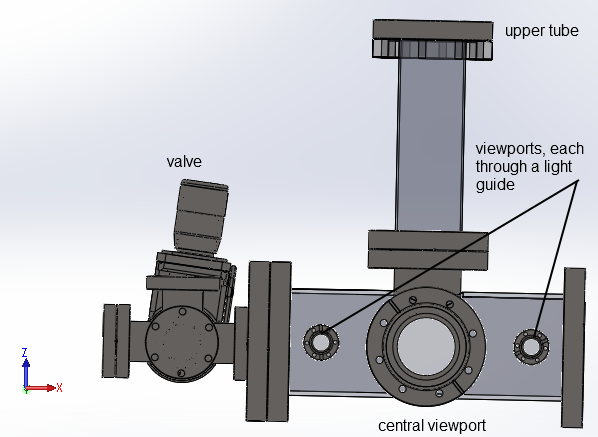
\includegraphics[width=0.4\textwidth,keepaspectratio]{chamber_front_names.PNG}
	\end{center}
	\begin{itemize}

		
		\item Measurements conducted with vacuum engine off.
		\item Maintenance of low pressure; leakage(volume) and the outgassing(surface).
		\pause
		\item CF vacuum chamber with light guides and three transparent windows in front.
		\item Measured pressure during the experiments is $P \approx 1\cdot 10^{−2} [pa]$
	\end{itemize}
	
\end{frame}




















\section{Summary and conclusion}
\begin{frame}{Study achievements}
	\begin{itemize}
		
		
		\item Explore possibilities of improving gravimetric measurements sensitivity and integration time. 
		\item Design a torsional pendulum with active motion damping. 
		\pause
		\item Results suggest that the amplitude could be damped up to the Brownian motion uncertainty limit. 
		%\item When damping beyond the thermal quantum uncertainty, damping effectively cools down the pendulum temperature.
		
		
	\end{itemize}
\end{frame}

\begin{frame}{Study contribution}
	\begin{itemize}
		
		\item Study contribution; with the right conditions, damping allows cooling up to the Brownian limit. 
		\item Resulting with higher gravimetric measurement sensitivity than current state of the art.
		\pause
		\item PID not the best control algorithm; linear approximation. 
		\item Next stage would have non linear motion approximation.
		\item Goal of damping beyond room temperature uncertainty. 
	\end{itemize}
\end{frame}

% frame 4
\begin{frame}{\hypertarget{frame:Radiation tourqe}{Radiation tourqe}}
	\begin{center}		
		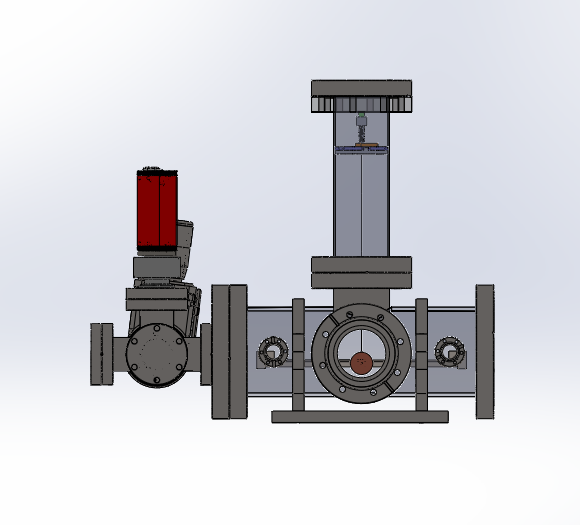
\includegraphics[width=0.4\textwidth,keepaspectratio]{total_chamber.png}
	\end{center}
	\begin{itemize}		
		\item Vacuum chamber is designed with two transparent windows with modulated light sources in front.
		\pause
		\item Incident light beam causes force on the surface, due to momentum exchange with the electromagnetic field.
		%\item The force depend on the relative angle, surface reflectance and absorbance and the incident light power.
		\pause
		\item With light perpendicular to a reflective surface $F  \approx\frac{2\eta\Theta}{{c}} $.
		\item Two light sources result with a modulated net tourqe.
		
	\end{itemize}
\end{frame}


\iffalse

\subsection[Basic Problem]{The basic problem that we have studed}

\begin{frame}{Slide Title \#1}
	\framesubtitle{Slide subtitle \#1}
	\begin{itemize}
		\item Use the \texttt{itemize} environment frequently.
		\pause
		\item Use short sentences and phrases.
		\pause
		\item In this presentation we use the \textbackslash{}\texttt{pause} macro.
	\end{itemize}
\end{frame}

\begin{frame}{Slide Title \#2}
	\begin{itemize}
		\item <1->You can define the order of appearance.
		\item <3->Like here.
		\item <2->This is the second item to appear.
	\end{itemize}
\end{frame}

\begin{frame}{Slide Title \#3}
	\begin{block}
		<1->{}
		\begin{itemize}
			\item Group without title.
			\item Appears for all slides.
		\end{itemize}
	\end{block}
	\begin{exampleblock}
		<2->{Group title}
		\begin{itemize}
			\item $e^{i\pi}=-1$.
			\item $e^{i\pi/2}=i$.
		\end{itemize}
	\end{exampleblock}
\end{frame}

%%
\subsection{Previous work}

\begin{frame}{Slide Title \#4}
	\begin{example}
		<1->First example. 
	\end{example}
	\begin{example}
		<2->Second example.
	\end{example}
\end{frame}

\begin{frame}{Slide Title \#5}
	\begin{center}
		Table example \\[12pt]
		\begin{tabular}{c||c|c|c|}
			& \textbf{col 1} & \textbf{col  2} & \textbf{col 3} \\
			\hline
			\hline
			\textbf{row 1} & 11 & 12 & 13 \\
			\hline
			\textbf{row 2} & 21 & 22 & 23 \\
		\end{tabular}
    \end{center}
\end{frame}

\begin{frame}{Slide Title \#6}
	\begin{center}
		Figure example \\[12pt]
		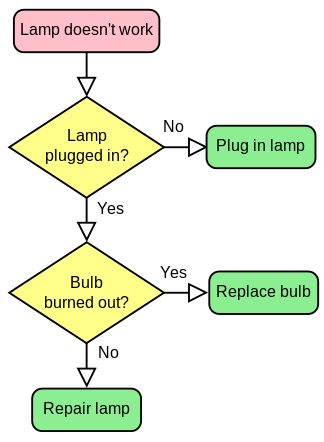
\includegraphics[width=0.35\textwidth,keepaspectratio]{LampFlowchart.png}
		\\
		\footnotesize(source: \textlatin{Wikipedia})
    \end{center}
\end{frame}

\begin{frame}{Slide Title \#7}
	\centering
	Math examples \\[12pt]
	\begin{equation}
        	B'=-\nabla \times E
	\end{equation}
	\begin{equation*}
        	E'=\nabla \times B - 4\pi j
	\end{equation*}
\end{frame}

%%%%
\section{Results / contribution}

%%
\subsection{Main results}

\begin{frame}{Summary}
   	\begin{alertblock}{Attention}
   		\textlatin{This is an important alert}
   	\end{alertblock}
\end{frame}

%
\subsection{Subsection title}

\begin{frame}{Summary}
	\begin{itemize}
		\item The \textcolor{red}{first main message} of our talk.
		\item The \textcolor{red}{second main message} of our talk.
		\item Maybe a \textcolor{red}{third message}, but ... no more.
	\end{itemize}
	\vskip0pt plus.5fill
	\begin{itemize}
		\item Conclusion.
	\end{itemize}
	\begin{itemize}
		\item Future work.
		\item Discussion.
	\end{itemize}
\end{frame}

\begin{frame}{References}
	\begin{thebibliography}{2}
		\beamertemplatebookbibitems
		\bibitem{Author1990}A.\ Author. \newblock\emph{Handbook of Everything}.\newblock
\textlatin{Some Press, \oldstylenums{1990}}.

		\beamertemplatearticlebibitems
		\bibitem{Someone2002}B.\ Author.\newblock On this and that\emph{.}
\newblock\emph{Journal on This and That}. 
\oldstylenums{2}(\oldstylenums{1}):\oldstylenums{50}--\oldstylenums{100}, 
\oldstylenums{2000}.
	\end{thebibliography}
\end{frame}
\fi
%%
\end{document}